%-------------------------
% Resume in LateX
% Author : Kevin Josue Hernandez Gomez
% License : MIT
%------------------------

\documentclass[letterpaper,11pt]{article}

\usepackage{latexsym}
\usepackage[empty]{fullpage}
\usepackage{titlesec}
\usepackage{marvosym}
\usepackage[usenames,dvipsnames]{color}
\usepackage{verbatim}
\usepackage{enumitem}
\usepackage[hidelinks]{hyperref}
\usepackage{fancyhdr}
\usepackage[english]{babel}
\usepackage{tabularx}
\usepackage{ragged2e}
\usepackage{graphicx}
\input{glyphtounicode}

\pagestyle{fancy}
\fancyhf{} % Clear all header and footer fields
\fancyfoot{}
\renewcommand{\headrulewidth}{0pt}
\renewcommand{\footrulewidth}{0pt}

% Adjust margins
\addtolength{\oddsidemargin}{-0.5in}
\addtolength{\evensidemargin}{-0.5in}
\addtolength{\textwidth}{1in}
\addtolength{\topmargin}{-.5in}
\addtolength{\textheight}{1.0in}

\urlstyle{same}

\raggedbottom
 
\raggedright
\setlength{\tabcolsep}{0in}

% Sections formatting
\titleformat{\section}{
  \vspace{-4pt}\scshape\raggedright\large
}{}{0em}{}[\color{black}\titlerule \vspace{-5pt}]

% Ensure that generate PDF is machine readable/ATS parsable
\pdfgentounicode=1

%-------------------------
% Custom commands
\newcommand{\resumeItem}[2]{
  \item\small{
    \textbf{#1}{: #2 \vspace{-2pt}}
  }
}

% Just in case someone needs a heading that does not need to be in a list
\newcommand{\resumeHeading}[4]{
    \begin{tabular*}{0.99\textwidth}[t]{l@{\extracolsep{\fill}}r}
      \textbf{#1} & #2 \\
      \textit{\small#3} & \textit{\small #4} \\
    \end{tabular*}\vspace{-5pt}
}

\newcommand{\resumeSubheading}[4]{
  \vspace{-1pt}\item
    \begin{tabular*}{0.97\textwidth}[t]{l@{\extracolsep{\fill}}r}
      \textbf{#1} & #2 \\
      \textit{\small#3} & \textit{\small #4} \\
    \end{tabular*}\vspace{-5pt}
}

\newcommand{\resumeSubSubheading}[2]{
    \begin{tabular*}{0.97\textwidth}{l@{\extracolsep{\fill}}r}
      \textit{\small#1} & \textit{\small #2} \\
    \end{tabular*}\vspace{-5pt}
}

\newcommand{\resumeSubItem}[2]{\resumeItem{#1}{#2}\vspace{-4pt}}

\renewcommand{\labelitemii}{$\circ$}

\newcommand{\resumeSubHeadingListStart}{\begin{itemize}[leftmargin=*]}
\newcommand{\resumeSubHeadingListEnd}{\end{itemize}}
\newcommand{\resumeItemListStart}{\begin{itemize}}
\newcommand{\resumeItemListEnd}{\end{itemize}\vspace{-5pt}}

%-------------------------------------------
%%%%%%  CV STARTS HERE  %%%%%%%%%%%%%%%%%%%%%%%%%%%%


\begin{document}

%----------HEADING-----------------
\begin{tabular*}{\textwidth}{l@{\extracolsep{\fill}}r}
  \textbf{\href{https://github.com/kjhg4589/curriculum.git}{\Large Kevin Josue Hernandez Gomez}} & Correo: \href{mailto:kjhg.45.89@gmail.com}{kjhg.45.89@gmail.com}\\
  \href{}{} & Telefono: \href{tel:+50254179967}{54179967} \\
\end{tabular*}

%-----------ABOUT ME-----------------
\section{Perfil Profesional}
  \begin{minipage}{0.15\textwidth}
    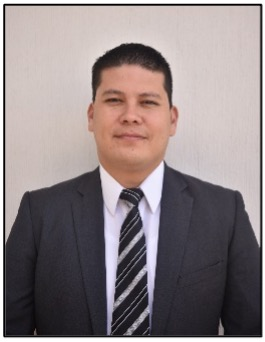
\includegraphics[width=0.9\linewidth]{img.jpg} 
  \end{minipage}
  \hfill
  \begin{minipage}{0.84\textwidth}
    \small
      \justifying
        Mi formación académica y familiar, junto con mi trayectoria profesional, han contribuido a construir un sólido ideal de vida basado en la ética, la responsabilidad y el respeto por la diversidad. Estos valores me impulsan a brindar un trato digno y respetuoso en cada entorno donde me desempeño, ya sea social o institucional. Cuento con una sólida claridad conceptual, habilidades para liderar y estructurar proyectos, facilidad para el trabajo en equipo y una destacada capacidad para gestionar relaciones interpersonales. Además, mantengo un compromiso constante con la actualización profesional y el aprendizaje continuo.
  \end{minipage}
%-----------EDUCATION-----------------
\section{Educacion}
  \resumeSubHeadingListStart
    \resumeSubheading
      {Universidad de San Carlos de Guatemala}{Guatemala, Guatemala}
      {Ingenieria en Ciencias y Sistemas; 9no Semestre}{Ene 2010 -- Presente}
    \resumeSubheading
      {Colegio Evangelico Mixto Integral}{Mixco, Guatemala}
      {Maestro de Educacion Primaria Urbana Mixta}{Ene 2005 -- Dic 2007}
  \resumeSubHeadingListEnd


%-----------EXPERIENCE-----------------
\section{Experiencia}
  \justifying
  \resumeSubHeadingListStart
    \resumeSubheading
      {Credito Hipotecario Nacional CHN}{Guatemala}
      {Analista de Aplicaciones}{Abr 2022 -- Presente}
      \resumeItemListStart
        \resumeItem{Sistema Integral de Seguros SISE}        
          {Participación activa en la migración del sistema de gestión de seguros SISE, pasando de su versión SISE2G (arquitectura cliente-servidor desarrollada en VB6) a SISE3G, una plataforma web desarrollada en C\#, utilizando Microsoft SQL Server como motor de base de datos.}
        \resumeItem{Modulo de Gastos Medicos}      
          {Responsable del desarrollo de múltiples herramientas para Gastos Médicos, contribuyendo significativamente a la eficiencia operativa y reducción de tiempos en la gestión de siniestros. (Java, Spring Boot, Keycloak)}
      \resumeItemListEnd
      
% --------Multiple Positions Heading------------
  %  \resumeSubSubheading
  %   {Software Engineer I}{Oct 2014 -- Sep 2016}
  %   \resumeItemListStart
  %      \resumeItem{Apache Beam}
  %        {Apache Beam is a unified model for defining both batch and streaming data-parallel processing pipelines}
  %   \resumeItemListEnd

%-------------------------------------------

    \resumeSubheading
      {B\&R Ingenieria de Sistemas INGESIS}{Guatemala, Guatemala}
      {Consultor de Soluciones}{Feb 2017 -- Mar 2022}
      \resumeItemListStart
        \resumeItem{Inxu Bancaseguros}
          {Participación en el desarrollo del sistema Banca-Seguros, una solución para la gestión de seguros masivos, utilizando Java con Spring 2 y Oracle 11g como motor de base de datos. El sistema es utilizado por entidades como Banco Promerica, ASSA Compañía de Seguros, Seguros Alianza, Scotiabank y Aseguradora SISA.}
        \resumeItem{Inxu FACE}
          {Desarrollo de la plataforma Inxu FACE, orientada a la generación de facturas electrónicas bajo el régimen FACE, utilizando Java EE y Sybase. El sistema se integra con los servicios de G4S para la emisión de comprobantes fiscales.}
        \resumeItem{Inxu FEL}
          {Implementación de Inxu FEL, una solución de facturación electrónica en el régimen FEL, construida con Java + Spring Boot y Oracle 12c, siguiendo una arquitectura de microservicios. El sistema se comunica con APIs de IFILE para la emisión de facturas.}
        \resumeItem{Inxu Microservicios}
          {Participación en la migración de los módulos del sistema de seguros hacia una arquitectura de microservicios, empleando Spring Boot y Java 11 en el backend, con MongoDB y Oracle como motores de base de datos, y Angular para el frontend.}        
      \resumeItemListEnd

    \resumeSubheading
      {Ingenieria Empresarial.}{Guatemala, Guatemala}
      {Analista Programador JR}{Mar 2015 -- Ene 2017}
      \resumeItemListStart
        \resumeItem{Control Admin}
          {Desarrollar Software contable dedicado al control y distribución de calzado, Se desarrollo utilizando sql server 2012 como motor de base de datos y power builder, el sistema se encuentra actualmente en empresas como LIMARCA, EUROZUELAS}
      \resumeItemListEnd

  \resumeSubHeadingListEnd


%-----------PROJECTS-----------------
\section{Proyectos}
  \resumeSubHeadingListStart
    \resumeSubItem{Backend Miniso}
      {Responsable del desarrollo del backend para la plataforma de e-commerce de Miniso, utilizando Java con Spring Boot y PostgreSQL como base de datos. El sistema fue integrado con servicios externos como NEO NET, Forza (gestión de paquetería) y Guatefacturas (facturación electrónica). Todo el desarrollo fue desplegado y gestionado en la infraestructura de AWS.}
  
  \resumeSubHeadingListEnd

%
%--------SKILLS------------
\section{Habilidades}
  \resumeSubHeadingListStart
    \item{
      \textbf{Languages}{:Java, C\#,  TypeScript, JavaScript, }
    }
    \item{
      \textbf{Bases de Datos}{: Oracle, MySql, PostgresSQL, MSSQL}
    }
    \item{
      \textbf{Tecnologias en la Nube}{: AWS, GCP, OCI}
    }
    \item{
      \textbf{Otras Tecnologias}{: Docker, Git, Suvbersion, Maven, Graddle, WebLogic, Jboss, WebSphere, IIS}
    }
  \resumeSubHeadingListEnd


%-------------------------------------------
\end{document}